\documentclass[16pt]{article}
\usepackage{fontspec}
\usepackage{parskip}
\usepackage{amsmath}
\usepackage{graphicx}
\usepackage{caption}
\usepackage{hyperref}
\usepackage{tabularx}
\usepackage{float}
\usepackage{subcaption}
\usepackage{algorithm}
\usepackage{algpseudocode}
\usepackage{algpascal}
\usepackage{geometry}
\usepackage{alltt}
\usepackage[backend=biber, citestyle=numeric, sorting=none]{biblatex}
\addbibresource{vde.bib}

\setmainfont{Noto Sans}
\hypersetup{urlcolor=blue, linkcolor=black, citecolor=black, colorlinks=true}
\author{James Engleback}

\begin{document}
\title{\textbf{VDE}}
\maketitle
\tableofcontents

\section{Abstract}
% ----------------
\section{Introduction}

\subsection{Background}
\subsubsection{Herbicide Resistant Crops}
Herbicide-resistant crops are important for global agriculture because they mitigate yield losses due to weeds and give farmers extra flexibility in their herbicide application programs, which is important to suppress emergence of herbicide-resistant weeds. 
% value statement

Herbicides kill plants by inhibiting key metabolic processes and their species-specificity is determined by susceptibility of herbicide target and their ability to  metabolize the herbicide. % herbicide overview
HPPD inhibitors are a key herbicide class that cause leaf bleaching and death in susceptible plants. 
HPPD inhibition  disrupts tyrosine catabolism which disrupts UV-protection via carotenoid production and photosynthetic electron shuttling via plastoquinone, leading to death by UV damage and radical toxicity. % HPPDs

Engineering HPPD-inhibitor resistance into plants have used the HPPD and metabolic enzymes from naturally resistant species like \textit{Avena fatua}, which employs cytochrome P450 Cyp72A1  to initiate metabolism of mesotrione by ring hydroxylation at $C_5$.
In this case, the $C_5$ hydroxylation acts as a target site for glutathione-S-transferases which conjugate glutathione to xenobiotics.
The glutathione conjugate tags the xenobiotic for sequestration in the cell vacuole, which neutralises the threat.

Engineered Cyp72A1 has been explored as a means of HPPD herbicide in soybean, which is an important target recipient for HPPD resistance traits. % cyp 72a1 & engineering attempts
%%%%% CYP71A1 stuff

\begin{figure}
	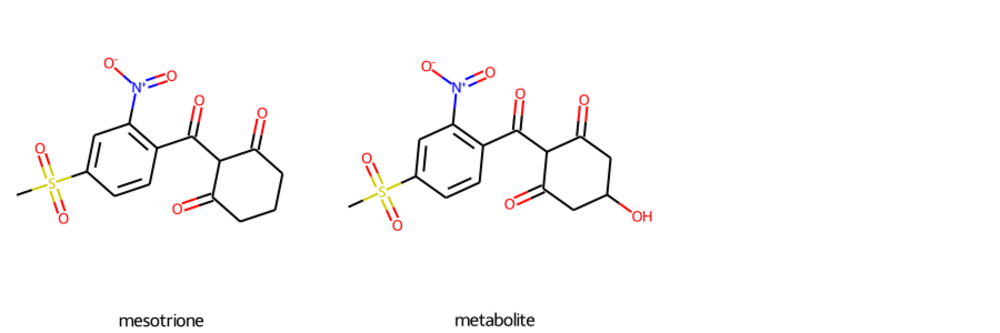
\includegraphics[width=\textwidth]{img/mesotrione+metabolite.png}
	\caption{\label{mesotrione} The HPPD inhibiting herbicide mesotrione and its primary metabolite 5-hydroxy-mesotrione in resistant strains of \textit{A. fatua}.}
\end{figure}

\subsubsection{Cytochrome P450s}
Cytochrome P450s are a ubiquitous class of heme-dependent oxido-reductases that are frequently involved in xenobiotic metabolism. % P450s overview
Bacterial P450s have been engineered to catalyse a range of xenobiotic biotransformations. 
The bacterial P450 BM3 from \textit{Bacillus megaterium} is one such bacterial P450 whose structure has been studied extensively. 
The A82F/F87V mutant has a broad substrate specificity, however it has no activity towards the HPPD herbicide mesotrione. % bacterial P450 engineering

\subsubsection{Virtual Directed Evolution}
Enzymes can be designed computationally using a genetic algorithm that evaluates the fitness of mutants by simulating the interaction between a target substrate and the predicted structure of the mutant. % computational enzyme edsign

The structure of a mutant can be predicted based on a template using techniques such as side-chain repacking by stochastic sampling from rotamer libraries and loop remodelling by cyclic coordinate descent. % structure pred - side chain repacking and loop ccd

% vde
Binding site interaction can be predicted using molecular docking, which attempts to predict likely protein-ligand binding conformations. 
A combination of the energy score and the conformation of docked molecules can be used to estimate likelihood of desirable reaction and therefore the fitness of a mutant. %score
In rounds of selection within a genetic algorithm, the fitness of a batch of mutants is evaluated by scoring desirability of protein-ligand binding, the fittest mutants are selected for breeding, in which mutants have elements of their genes recombined are further mutated, then the cycle repeats.   % genetic algorithms

\subsection{Technologies Used}
\subsubsection{Directed Evolution}
\subsubsection{Structure-Based Design}
\subsubsection{Protein Structure Prediction}
\subsubsection{Docking}
\subsubsection{Sequence Optimization Algorithms}
\subsubsection{Overview of this work}
\subsubsection{Engineering Problem}
\subsection{Overview of this Work}

Here, in attempt to engineer a mutant of the Cytochrome P450 BM3 to hydroxylate mesotrione at the $C_5$ position is made by developing a \textit{VDE} system, deploying it at scale on cloud infrastructure and identification on clusters of putatively active mutants.
% ----------------
\section{Methods}

The project was operated as a  \texttt{git} repository which can be found here: \href{https://github.com/jamesengleback/vde}{https://github.com/jamesengleback/vde}.
The structure of the directory is:

\begin{alltt}
docs/         # write up for this document and markdown docs
nb/           # jupyter notebooks used for data analysis
scripts/      # scripts to create and configure cloud machines to run algorithm on
vde/          # the vde algorithm configured to optimize BM3 for desirable mesotrione binding
\end{alltt}

This section details the implementation of this project:
\begin{itemize}
	\item The project is dependent on a \texttt{python} packagge \texttt{enz}, developed here for protein structure prediction and molecular docking to predict the behaviour of mutants; described in \ref{enz}.
	\item A score function that attempts to predict the likelihood of a $C_5$ hydroxylation of mesotrione is described in section \ref{scorefn}.
	\item A genetic algorithm to optimize the sequence of BM3 mutants is discussed in section \ref{ga} 
	\item Section \ref{cloud} describes execution of the algorithm at scale on cloud infrastructure.
\end{itemize}


% ---------------- enz ---------------- 
\subsection{\texttt{enz} \label{enz}}

Abstraction and modularization of protein structure prediction and molecular docking was important for reducing complexity of experiments and developability of the algorithm.
To this end the \texttt{python} package \texttt{enz} was created, an \textit{Application Program Interface (API)} wrapper around the \textit{PyRosetta} \cite{chaudhury2010pyrosetta} protein structure prediction software and the \textit{Autodock VINA} \cite{trott2010autodock} binary, as well as utilities to handle file format conversion using \textit{OpenBabel} \cite{o2011open}.
The package is modular enough to allow replacement of its functionality-providing back-ends according to a users requirements and is hosted at \href{https://github.com/jamesengleback/enz}{https://github.com/jamesengleback/enz}.

\texttt{enz} performs the following functions:
\begin{itemize}
	\item \textbf{Protein Structure Prediction:} \texttt{enz} uses side chain repacking \cite{dunbrack1993backbone} functionality from \textit{PyRosetta} for template-based structure prediction. 
		This functionality is provided by \textit{Pyrosetta}.
	\item \textbf{Docking:}
	\item \textbf{Return new atomic coordinates:} via \texttt{pandas} DataFrames, which can be used to score pose configurations.
\end{itemize}

The user-exposed command set is minimal so programs written using \texttt{enz} can be short.

\subsection{Score function \label{scorefn}}
Mutants were to be scored on the basis of presumed likelihood of a mutant being able to 5-hydroxylate mesotrione based on the docked mesotrione poses and their predicted binding energies.
Given that the likelihood of electron transfer from the heme iron to the recipient carbon atom decreases with distance $d$ at a rate $\frac{k}{d^6}$ where $d$ is distance between the target and the gheme iron \cite{moser2008distance}.

The heuristic currently employed to estimate the desirability of each set of $m$ docking results is described in equation \ref{scoreeqn}: % heuristic
\begin{equation}\label{scoreeqn}
	score = \frac{1}{n}\sum^{n}_{i\in m} \Delta G_{i} \times d_{i}
\end{equation}
where $\Delta G$ is a free energy estimation of the interaction calculated by \textit{Autodock VINA} (given in \textit{kcal/mol}) and $d$ is the distance between the heme iron and the $C_{5}$ of mesotrione for each of $m$ binding poses \textbf{(figure \ref{score})}. 

\begin{figure}
	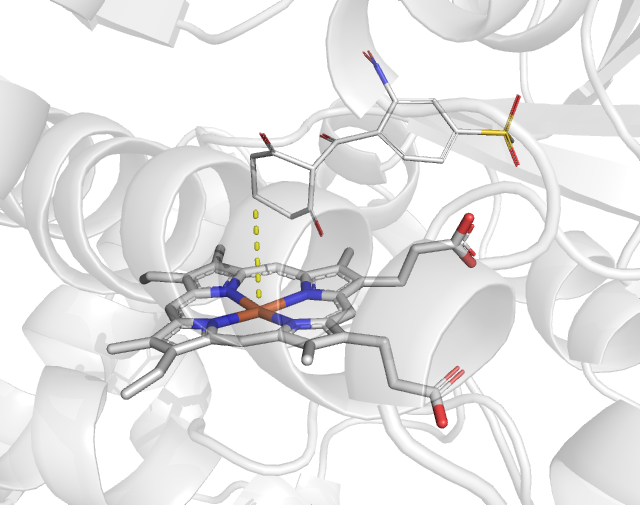
\includegraphics[width=\textwidth]{img/score.png}
	\caption{\label{score} - Distance $d$  between carbon $C_5$ of mesotrione and the heme iron of BM3, used in the fitness score (\AA) marked by a yellow dashed line.}
\end{figure}

\subsection{Genetic Algorithm \label{ga}}

A simple genetic algorithm \textit{(GA)} was used for sequence optimization during \textit{VDE}.
The \textit{GA} was implemented in pure \texttt{python} and its built-in modules.

In this case, the \textit{GA} repeated the following steps in each iteration:
\begin{enumerate}
	\item \textbf{Initialize mutant population:} From the template sequence, generate $p$ mutants each with one random point mutation.
	\item \textbf{For $n$ Iterations:}
		\begin{enumerate}
	\item \textbf{Evaluate \textit{fitness} of each mutant:\label{gaeval}} Using multiprocessing, evaluate the score for each mutant in parallel, returning a mapping of sequences to respective scores.
	\item \textbf{Select for best $\frac{1}{m}$ mutants:} where $\frac{1}{m}$ is the survival rate in each iteration.
	\item \textbf{Repopulate gene pool by crossover and point mutation of selected mutants:} where two random members of the surviving mutants $a$ and $b$ are crossed by recombining sequences at a random cut point and introducing additional random point mutation.
		Repeat $p$ times.
		\end{enumerate}
\end{enumerate}

\alglanguage{pseudocode}
\begin{algorithm}
	\caption{\label{pseudocode}: A genetic algorithm}
	\
	\begin{algorithmic}
		\Procedure{GA}{$seq,popsize,n_{iter}$}
		\For{$p_i:=1, p_i \leq popsize$}
			\State $pop_i := mutate(seq)$ 
		\EndFor
		\For{$i:=1, i \leq n_{iter}$}
			\ForAll{$mutant_j \in pop$}
				\State $fitness_j := fn(mutant_j)$
			\EndFor
		\EndFor
		\EndProcedure
	\end{algorithmic}
\end{algorithm}

Algorithm \ref{pseudocode} is implemented in \texttt{python} in the file \texttt{vde/ga.py} and makes use of multiprocessing to parallelise evaluations of a function.

\subsection{Main Function \label{main}}
The program in \texttt{vde/main.py} executes the main functionality of \textit{VDE}.
It executes iterations of the genetic algorithm \ref{ga} where the evaluation function for a $sequence $ is:

\begin{algorithm}
	\caption{\label{fitness}: One fitness evaluation}
	\
	\begin{algorithmic}
		\Procedure{Evaluate Mutant}{$sequence$}
		\State structure = map\_refold(sequence, pdb=\texttt{4KEY.pdb}) \Comment{Predict mutant structure \cite{dunbrack1993backbone} \cite{chaudhury2010pyrosetta}.}
		\State docking poses = dock(structure, mesotrione) \Comment{\cite{trott2010autodock}}
		\State fitness = score(docking poses) \Comment{Using score \ref{scorefn}}
		\State \textbf{Return} fitness
		\EndProcedure
	\end{algorithmic}
\end{algorithm}
\subsection{Cloud Deployment \label{cloud}}
% ----------------
\section{Results}

% ----------------
\section{Discussion and Future Work}


\printbibliography
\end{document}
